\documentclass[a4paper, 10pt]{article}
\hyphenpenalty=8000
\textwidth=125mm
\textheight=185mm

\usepackage{graphicx}
\usepackage{alltt}
\usepackage{amsmath}
\usepackage[hidelinks, pdftex]{hyperref}
\usepackage{cite}
\usepackage{float}  % Se añade el paquete float para controlar la posición de las imágenes

\pagenumbering{arabic}
\setcounter{page}{1}
\renewcommand{\thefootnote}{\fnsymbol{footnote}}
\newcommand{\doi}[1]{\href{https://doi.org/#1}{\texttt{https://doi.org/#1}}}

\begin{document}

\begin{center}
Nonlinear Analysis: Modelling and Control, Vol. vv, No. nn, YYYY\\
\copyright\ Vilnius University\\[24pt]
\LARGE
\textbf{Simulación y animación de un punto en una escena 2D utilizando Python}\\[6pt]
\small
\textbf {Diego Alzate, Aris Avila, Julieth Gutierrez}\\[6pt]
IE INFOTEP, Ciénaga, Magdalena \\[6pt]
Recibido: 03 marzo de 2025\quad\quad
\end{center}

\begin{abstract}
Este informe detalla el desarrollo de una simulación en Python de un rectángulo y un punto sobrepuesto a este mismo.
\vskip 2mm

\textbf{Palabras clave:} animación, Python, Google Colab, simulación 2D, animación.
\end{abstract}

\section{Introducción}\label{s:1}
Este informe describe el desarrollo al simular la representación de un rectángulo y un punto, de la modificación de ambos y la animación de movimiento del punto dentro de la escena.

\section{Objetivos de la actividad}\label{s:2}
El objetivo de esta actividad es desarrollar la representación gráfica de un rectángulo donde el tamaño y el color son recibidos por parámetros, un punto ubicado de manera aleatoria y también poder cambiar estos mismos parámetros. Además, de esta manera se refuerzan conceptos y prácticas en POO.

\section{Descripción de la actividad}\label{s:3}
Para desarrollar la actividad, utilizamos la clase \texttt{Escena} que contiene un rectángulo de fondo y un punto que en primera instancia se ubica de manera aleatoria en esta. Ambas figuras pueden cambiar ciertos parámetros mediante las funciones \texttt{desplazar\_punto}, \texttt{cambiar\_escena}, y también el punto puede moverse de manera animada a cierta velocidad y dirección mediante \texttt{simular}, los cuales son recibidos por parámetros. Se implementó la animación utilizando la clase \texttt{FuncAnimation} de \texttt{matplotlib}. Debido a las limitaciones de Google Colab para manejar animaciones interactivas, se generó un video HTML de la animación para poder visualizarla.

\section{Gráficas de resultados}\label{s:4}

\begin{figure}[H]
\centering
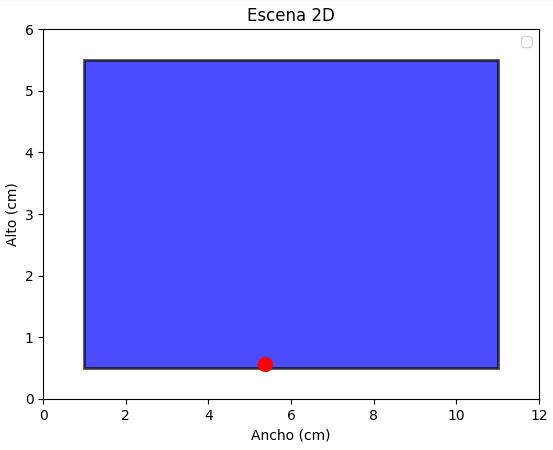
\includegraphics[width=5.8cm]{grafica1.png} % Coloca el nombre de la imagen aquí
    \caption{Creacion de escena con un rectangulo de 10x5 color azul.}
\label{fig:1}
\end{figure}

\begin{figure}[H]
\centering
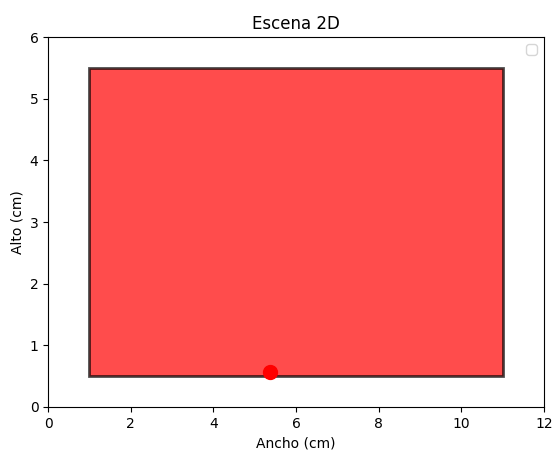
\includegraphics[width=5.8cm]{grafica2.png} % Nombre de la segunda imagen
\caption{Se cambio el color del rectangulo a rojo.}
\label{fig:2}
\end{figure}

\begin{figure}[H]
\centering
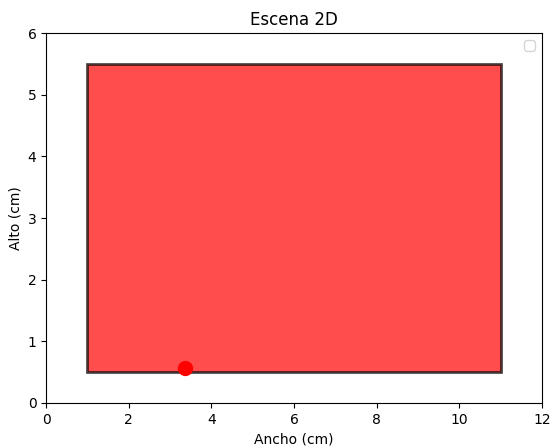
\includegraphics[width=5.8cm]{grafica3.png} % Nombre de la tercera imagen
\caption{Se movio el punto a la izquierda 2cm.}
\label{fig:3}
\end{figure}

\begin{figure}[H]
\centering
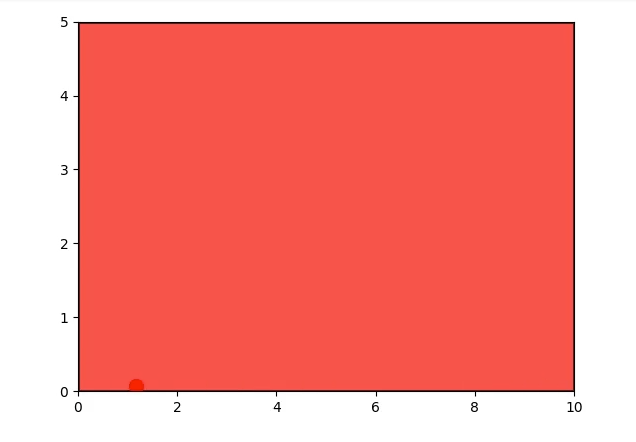
\includegraphics[width=5.8cm]{grafica4.png} % Nombre de la cuarta imagen
\caption{El punto rebotando en el lado izquierdo.}
\label{fig:4}
\end{figure}

\section{Análisis de la gráfica}\label{s:5}
En la figura \ref{fig:1} se ve la representación de la figura, en la figura \ref{fig:2} el cambio del color del rectángulo, en la figura \ref{fig:3} el desplazamiento del círculo a la izquierda, y la figura \ref{fig:4} es una foto de la animación que se puede ver al ejecutar el código en Google Colab.

\section{Conclusiones}\label{s:6}
Se concluye que **Google Colab no soporta animaciones interactivas** en tiempo real debido a las limitaciones de su backend gráfico. Sin embargo, se encontró una solución alternativa utilizando la conversión de la animación en un video HTML. Esta solución permite que la animación sea visible dentro de Google Colab, aunque no sea interactiva en tiempo real.

\section{Referencias}\label{s:7}
\begin{itemize}
    \item Python Classes. \href{https://docs.python.org/es/3.13/tutorial/classes.html}{https://docs.python.org/es/3.13/tutorial/classes.html}
    \item Video tutorial sobre la creación de clase con un rectangulo en Python. \href{https://www.youtube.com/watch?v=0V4NLnKcz94}{https://www.youtube.com/watch?v=0V4NLnKcz94}
    \item Introducción a las formas básicas de Python. \href{https://josejuansanchez.org/processing-python/formas_bsicas.html}{https://josejuansanchez.org/processing-python/formas_bsicas.html}
\end{itemize}

\end{document}
